\section{Thermal shield vibrations}\label{sec:4:thermal-vibrations}

\begin{figure}[!htbp]
  \centering
  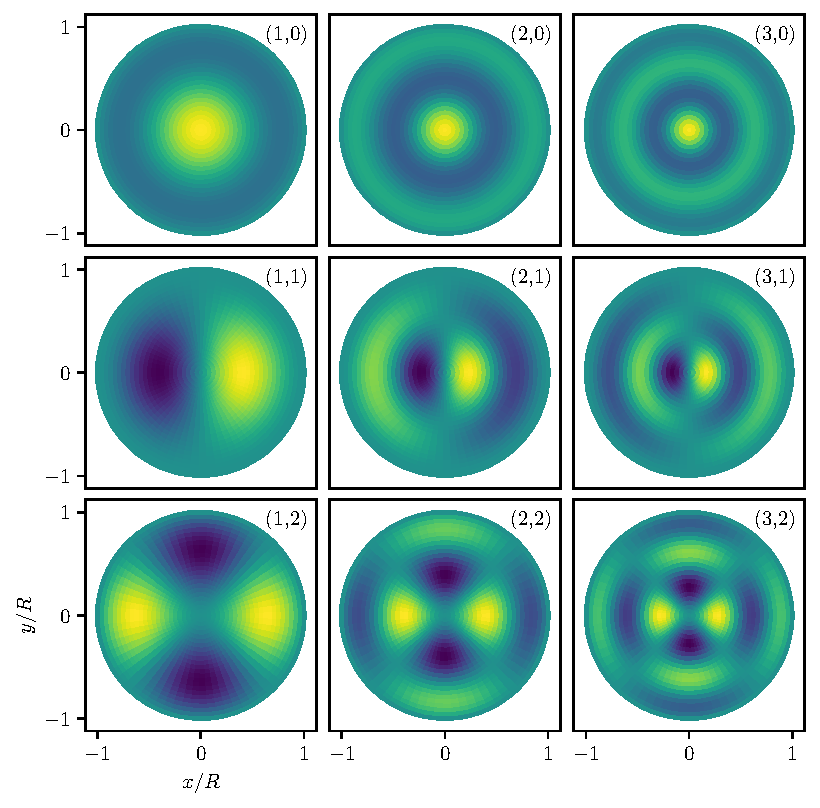
\includegraphics[width=\textwidth]{./../figures/vibrations/vibrational-modes.pdf}
  \caption{Normalized shape of the vibrational modes $(k,l)$ of a vibrating spherical plate fixed at the edge with $R/d = 1000$.}
  \label{fig:4:vibrational-modes}
\end{figure}



\begin{equation}
  \op{H} = \hbar \omega \left(\op{a}^\dagger\op{a} + \frac{1}{2}\right) + \tilde{g}_A(\op{z}) \ketbra{\psi_A} + \tilde{g}_B(\op{z}) \ketbra{\psi_B}
\end{equation}

Solution:
\begin{equation}
  \rho(t) = \frac{1}{2}\begin{pmatrix}
    1 & e^{-i\varphi(t)}e^{-\gamma(t)}\\
    e^{i\varphi(t)}e^{-\gamma(t)} & 1
  \end{pmatrix}
\end{equation}
with the phase
\begin{equation}
  \varphi(t) = \frac{1}{\hbar^2\omega^2} \left(\sin(\omega t) - \omega t\right) \left(g_A^2 - g_B^2\right)
\end{equation}
and the decoherence term
\begin{equation}
  \gamma(t) = \frac{4(g_A - g_B)^2}{\hbar^2 \omega^2} \sin(\frac{\omega t}{2}) \left[\bar{n} + \frac{1}{2}\right]
\end{equation}

\begin{figure}[!htbp]
  \centering
  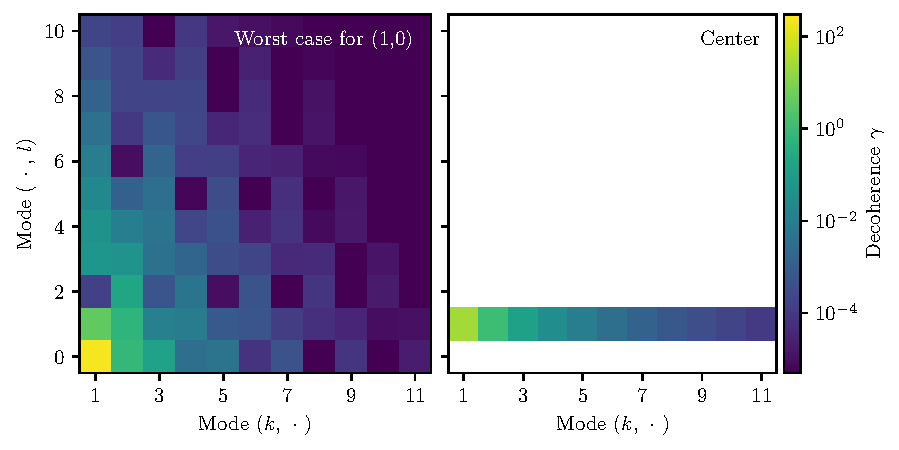
\includegraphics[width=\textwidth]{./../figures/vibrations/decoherence-analytical.pdf}
  \caption{Maximum decoherence $\gamma$ at $4\si{K}$ for all modes if the cat-state is placed \textbf{left:} at the point with maximum gradient of the mode $(1,0)$ and \textbf{right:} in the center of the plate. It becomes evident, that only a few low modes play an actual role for the total dephasing.}
  \label{fig:4:}
\end{figure}